\chapter{Hashing}
\label{chapter-hashing}
Hashing is one of the approaches designed for the efficient solving of the dictionary problem. Various implementations differ in many ways. However usage of a hash function and a quickly accessible table, typically represented by an array, is common to most of them. Every hash function transforms the elements of the universe into the addresses of the table.

Represented sets are always small when compared to the size of the universe. In order to prevent waste of space we are forced to use tables as small as possible. Typically the size of the hash table containing the represented elements is chosen so that it is comparable to the size of the stored set. 

The fact that the hash table is much smaller than the universe and any two elements may represented means that the elements may share the same address after hashing. This event is called a \emph{collision}. For hashing it is very important how collisions are handled. This is also the most interesting distinctive feature for distinct hashing models. In fact, collision handling is crucial when determining the time complexity of the scheme.

When two elements collide they should be stored in a single \emph{bucket}, cell of the hash table. A bucket is often represented by the simplest data structure possible. For instance, a singly linked list should be sufficient in many cases. More sophisticated schemes, like perfect hashing, represent every chain in another hash table without collisions.

The find operation of a hash table works in the following way. Every element is placed as an argument for the hash function. The element's address is then computed and used as an index of the hash table. Then we look into the bucket lying at the returned address if the element is stored inside or not.

\begin{figure}
  \centering
    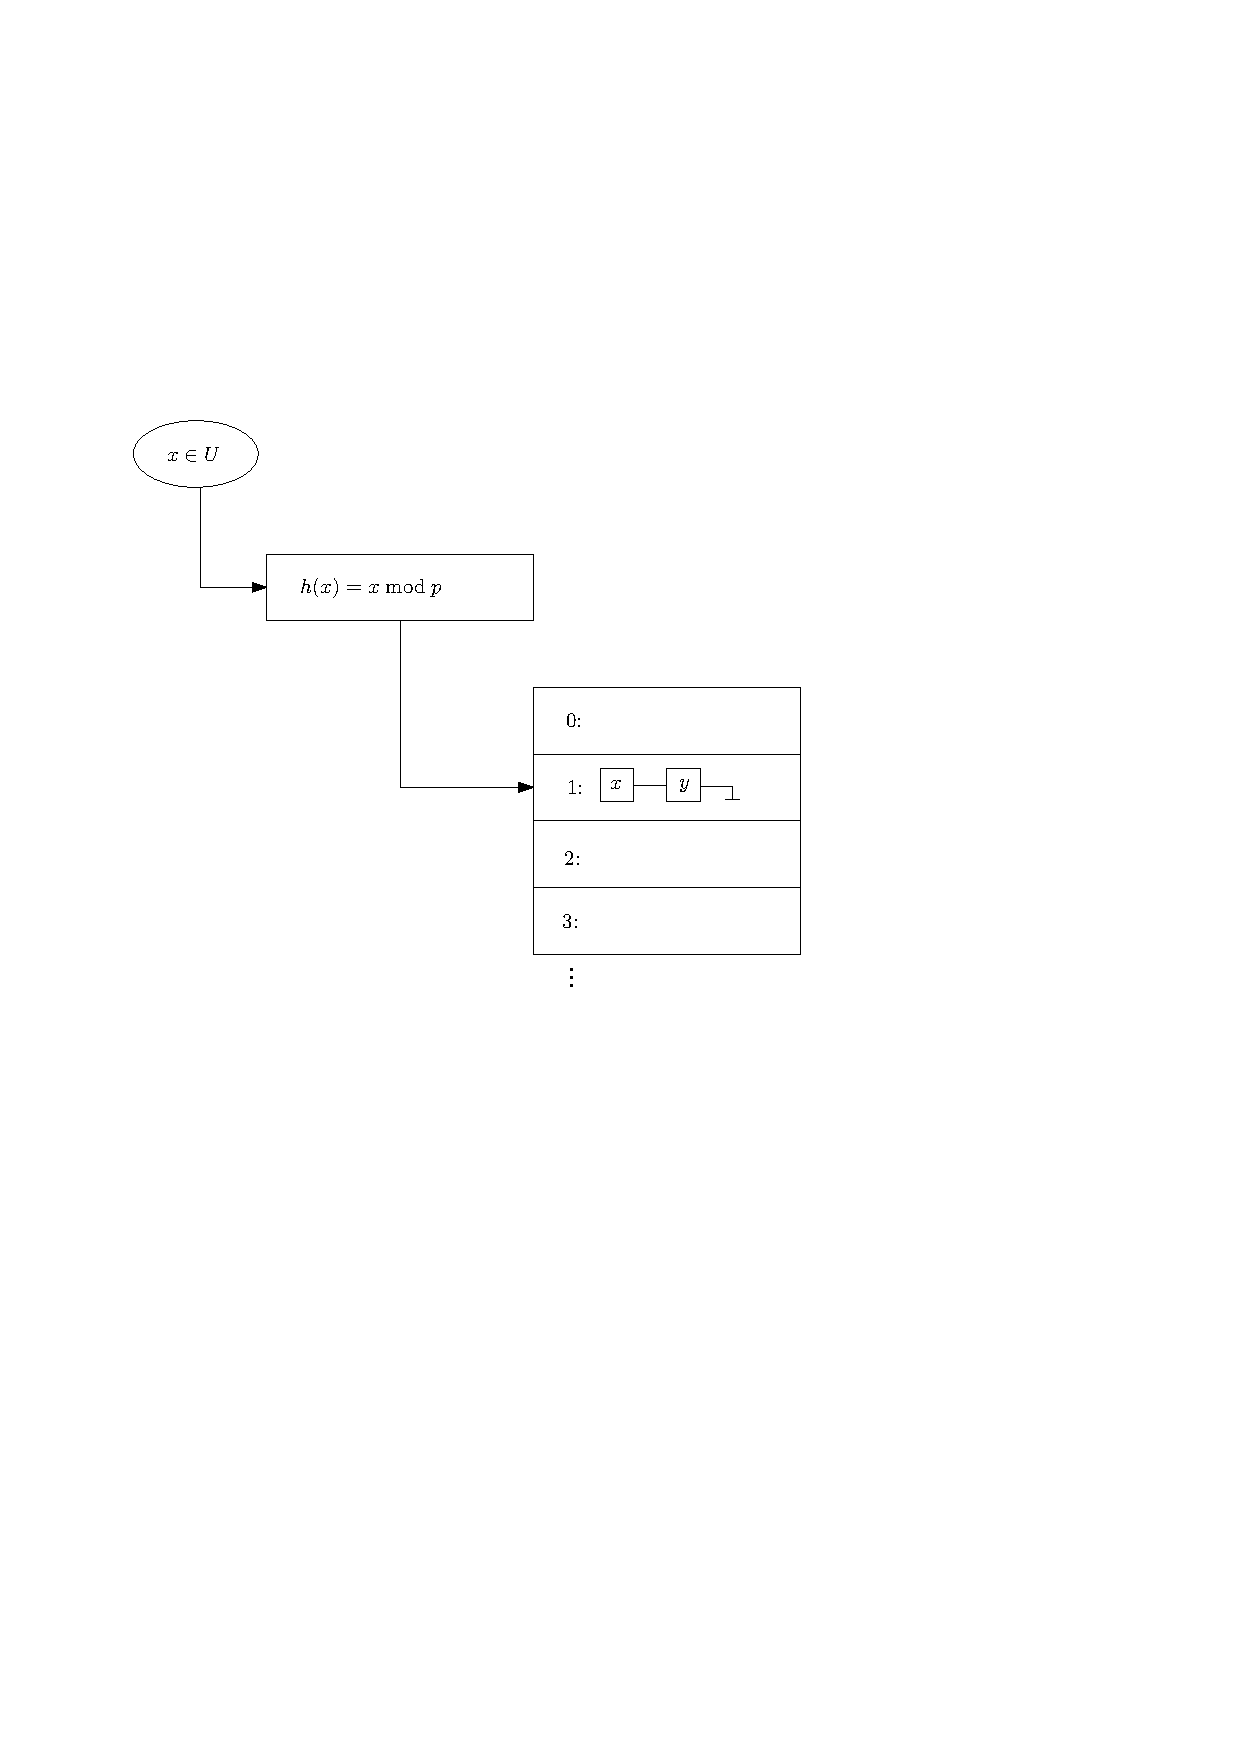
\includegraphics[width=0.5\textwidth]{images/hash_table}
  \caption{Concept of a hash table.}
\end{figure}

If buckets are represented by linked lists, then the expected time of the find operation is proportional to one half of the length of the list.
\begin{lemma}
\label{lemma-expected-list-time}
Let $S$ be a set represented by a linked list. Assume that for every element $x \in S$: \[ \Prob{x \text{ is argument of the find operation}} = \frac{1}{|S|} \text{.} \] Then the expected time of the find operation is $\frac{|S| + 1}{2}$.
\end{lemma}
\begin{proof}
Let $x_i \in S$ be the $i$-th element of the list, $1 \leq i \leq |S|$. Time to find the element $x_i$ inside the list equals $i$. The expected time of the find operation can be expressed directly from its definition
\[
\begin{split}
\Expect{\text{time of the find operation}} 
	& = \displaystyle\sum_{i = 1}^{|S|} i \Prob{x_i \text{ is the argument of the find operation}} \\
	& = \frac{\sum_{i = 1}^{|S|}{i}}{|S|} = \frac{|S|(|S| + 1)}{2 |S|} = \frac{|S| + 1}{2} \text{.}
\end{split}
\]
\end{proof}

As seen in the previous lemma the time complexity of an operation needs not to be measured by its worst case time. Compare $|S|$, which is the worst case, to the expected value $\frac{|S| + 1}{2}$ which is better. Considering only the worst case times does not tell much about the structure's real behaviour. We should use probability based characteristics that give more accurate results. These characteristics include the expected operation's time or its expected worst case time which is usually far more difficult to analyse. For hashing this difference means an asymptotic improvement.

\section{Formalisms and Notation}
\label{section-notation}
Notation and formalisms that mathematically describe a hash table are crucial part of an exact analysis. Assume that we are hashing a \emph{universe} $U$ on a \emph{hash table} of size $m$. The table consists of buckets each having its unique address. The addresses are usually quite simple. When the table consists of $m$ buckets the addresses are just $0, \dots, m - 1$. Buckets are always identified by their addresses and thus we can refer to the set $B = \{0, \dots, m - 1\}$ as a hash table.

Universe consists of all the representable elements, examples include the objects of a programming language, strings over an alphabet, numbers or anything else. Hash function is a way to transform these elements into an address of the table, usually a natural number. Hash function $h$ can be described by a function $h: U \rightarrow B$. The other requirements placed on the function $h$ are discussed later.

The letter $S$ typically denotes the \emph{stored set}. We often refer to the variable $n$ as to the size of the stored set, $n = |S|$. As already mentioned we always assume that $S \subset U$ and $|S| \ll |U|$.

Since the universes are really large, recall the previous examples, sizes of the tables are much smaller when compared to those of the universes. Space waste is typically caused by allocating a large table containing many empty buckets. The definition of the table's \emph{load factor} allows an exact analysis of the phenomena connected with the table's filling -- its performance or waste of space.

\begin{definition}[Load factor]
\label{definition-load-factor}
Let $n$ be the size of the represented set and $m$ be the size of the hash table. The variable $\alpha$ defined as \[ \alpha = \frac{n}{m} \] is called the \emph{load factor} of the table.
\end{definition}

To take control of the table's overhead it is sufficient to keep the load factor in a predefined interval. Not only the empty buckets cause troubles. The overfilled ones are another extreme especially if there are too many collisions.
\begin{definition}[Collision]
\label{definition-collision}
Let $h$ be a hash function and $x, y \in U$ be two distinct elements. We say that the elements $x$ and $y$ \emph{collide} if $h(x) = h(y)$.
\end{definition}

Above all the collision handling is what differentiates distinct hash tables and determines their performance.

To completely explain the notation we have to mention that we refer to the function $\log$ as to the binary logarithm. The function $\ln$ denotes the natural logarithm.

\section{Assumptions of Classic Hashing}
\label{section-assumptions}
In Lemma \ref{lemma-expected-list-time} we computed the expected time of the find operation and used it as a measure of its time complexity. Known probability distribution of the input enables us to compute the expected value. For the lemma we assumed the uniform distribution. In hashing similar situation occurs. If we want to find the expected results, then we need corresponding probabilistic assumptions on the input. The assumptions we make may be found in \cite{VK-skripta} or in \cite{DBLP:books/sp/Mehlhorn84}. They are similar to ours.
\begin{itemize}
\item Hash function $h$ distributes the elements of universe uniformly across the hash table:
\[
||h^{-1}(x)| - |h^{-1}(y)|| \leq 1 \text{ for every }x, y \in B \text{.}
\]
\item Every set has the same probability of being stored among the sets of the same size:
\[
\Prob{S \text{ is stored}} = \frac{1}{\dbinom{|U|}{|S|}} \text{ for every set } S \subset U \text{.}
\]
\item Every element of the universe has the same probability of being an argument of an operation:
\[
\Prob{x \text{ is used as an argument of an operation}} = \frac{1}{|U|} \text{ for every } x \in U \text{.}
\]
\end{itemize}

These assumptions provide us with a probabilistic model for the average case analysis of classic hashing.

\section{Separate Chaining}
Separate chaining \cite{The-art-of-computer-programming}, \cite{DBLP:books/sp/Mehlhorn84} and \cite{DBLP:books/sp/MehlhornS2008} may be considered the most basic hash table implementation. However, it provides a sufficient framework for illustration of various problems and analyses. Separate chaining usually utilises one hash function mapping elements to an address -- an index of the array representing the hash table. Every represented element is stored within a bucket given by its hash address. Every bucket is represented by a singly linked list. 

Separate chaining, like the other classic models of hashing, is quite dependent on the stored input. The previous assumptions are required for its average case analysis. This model assumes hashing of the universe $U = \{0, \dots, N - 1\}$ for $N \in \mathbb{N}$ into a table of size $m$. Number $m$ is much smaller then $N$ and moreover it is chosen to be a prime. Primality of $m$ improves the ability of the hash function to uniformly distribute the stored set across the table.  The following example clarifies why primality is important for the choice of $m$.

\begin{example}
Consider the set $S = \{5n \setdelim n \in \{0, \dots, 5\} \}$ and a table consisting of $10$ buckets. Set $S$ contains only 6 elements, so the table's load factor equals $0.6$. If we use function $x \bmod 10$, then it maps the elements of the set $S$ just onto two addresses, $0$ and $5$. The hash table is not used effectively. Choosing $m$ to be a prime number improves the results but is not a remedy.
\end{example}

The apparent disadvantage of classic hashing is usage of a single hash function known in advance. For example if  the stored set $S$ is chosen, by an adversary, so that $S \subseteq f^{-1}(b)$ for a single bucket $b \in B$, we run into problems. Because our assumptions say that the probability of having such an input is quite low, these inputs may be neglected.

To illustrate how separated chaining works the algorithms are presented. Although the model is quite simple the subroutines regarding the singly linked lists are not discussed. They are considered elementary enough. We remark that the running time is proportional to length of the represented chain. Also notice that the insert procedure has to check whether the element is already stored inside the list else it can be stored twice. 

\begin{algorithm}[H]
\caption{Find operation of the separate chaining.}
\label{algorithm-find-separate-chaining}
\floatname{algorithm}{Procedure}
\begin{algorithmic}
\REQUIRE $x \in U$
\STATE $h = h(x)$
\STATE
\IF {$T\left[h\right] \text{ contains } x$}
	\RETURN \textbf{true} \COMMENT{operation is successful}
\ELSE
	\RETURN \textbf{false} \COMMENT{operation is unsuccessful}
\ENDIF
\end{algorithmic}
\end{algorithm}

\begin{algorithm}[H]
\caption{Insert operation of the separate chaining.}
\label{algorithm-insert-separate-chaining}
\floatname{algorithm}{Procedure}
\begin{algorithmic}
\REQUIRE $x \in U$
\STATE $h = h(x)$
\STATE
\IF {$T\left[h\right] \text{ does not contain } x$}
	\STATE insert $x$ into chain $T[h]$
\ENDIF
\end{algorithmic}
\end{algorithm}

\begin{algorithm}[ht]
\caption{Delete operation of the separate chaining.}
\label{algorithm-delete-separate-chaining}
\floatname{algorithm}{Procedure}
\begin{algorithmic}
\REQUIRE $x \in U$
\STATE $h = h(x)$
\STATE
\IF {$T\left[h\right] \text{ contains } x$}
	\STATE remove $x$ from chain $T[h]$
\ENDIF
\end{algorithmic}
\end{algorithm}

\begin{theorem}[Average case of the separate chaining]
Let $\alpha > 0$ be the load factor of the hash table resolving collisions by separate chaining. Then the expected time of the successful find operation converges to $1 + \frac{\alpha}{2}$ and to $e^{-\alpha} + \alpha$ in the unsuccessful case.
\end{theorem}
\begin{proof}
The theorem is proved in \cite{DBLP:books/sp/Mehlhorn84}.
\end{proof}

Various modifications of separate chaining are known. If the universe is an ordered set then ordering the elements in chains monotonously may bring a speedup. This is caused by the fact that the operations concerning the chains do not have to iterate throughout the whole list and stop earlier. 

There is a modification utilising the move to front principle \cite{723912}. This principle is motivated by the rule of the locality of reference \cite{DBLP:books/aw/AhoSU86}. The rule says that whenever an element is accessed, it is very likely that it is going to be accessed again in a short future. Therefore it is quite convenient to put the last accessed element to the front of the list so that it is accessed fast.

Another set of modifications changes the representation of chains. They are no longer represented by common linked lists since their cache behaviour \cite{1200662} is poor as stated in \cite{Rubin99virtualcache}. The chains are stored directly in the hash table. So when resolving a collision an empty place in the hash table is taken. There are problems connected with this approach that need to be solved. Above all chains may not be merged together. This appears when a new chain should be started but the place of the first element is already taken. It may be solved by moving the element, not belonging to the chain, to another empty place. To perform the replacement quickly we are forced to use double linkage. Or, instead of using doubly linked lists, at every address an additional begin pointer may point to the first element of the chain. In addition, we have to deal with the fact that schemes using only the hash table suffer from bad behaviour when the load factor is almost one. And of course a uniform random choice of an empty bucket has to be provided when prolonging a chain.

\section{Coalesced Hashing}
In coalesced hashing, the chains of colliding elements are also stored directly in the hash table. However, they are allowed to fuse together. Every chain is represented by a singly linked list. The simpler methods such as LISCH and EISCH do not use any special additional memory. In addition, the EISCH method utilises the move to front rule. Methods such as LICH, EICH and VICH use the additional memory which is not directly addressable by the hash function. Collision resolution uses the additional memory to store growing chains. When an empty place for a colliding element is needed, it is first sought in the additional memory. Only if the special memory is full, then the addressable memory is used. The methods are distinct in a way they use the move to front rule. The EICH method always obeys it, VICH uses it only in the addressable memory and the LICH method does not obey the rule at all.

\begin{figure}
  \centering
    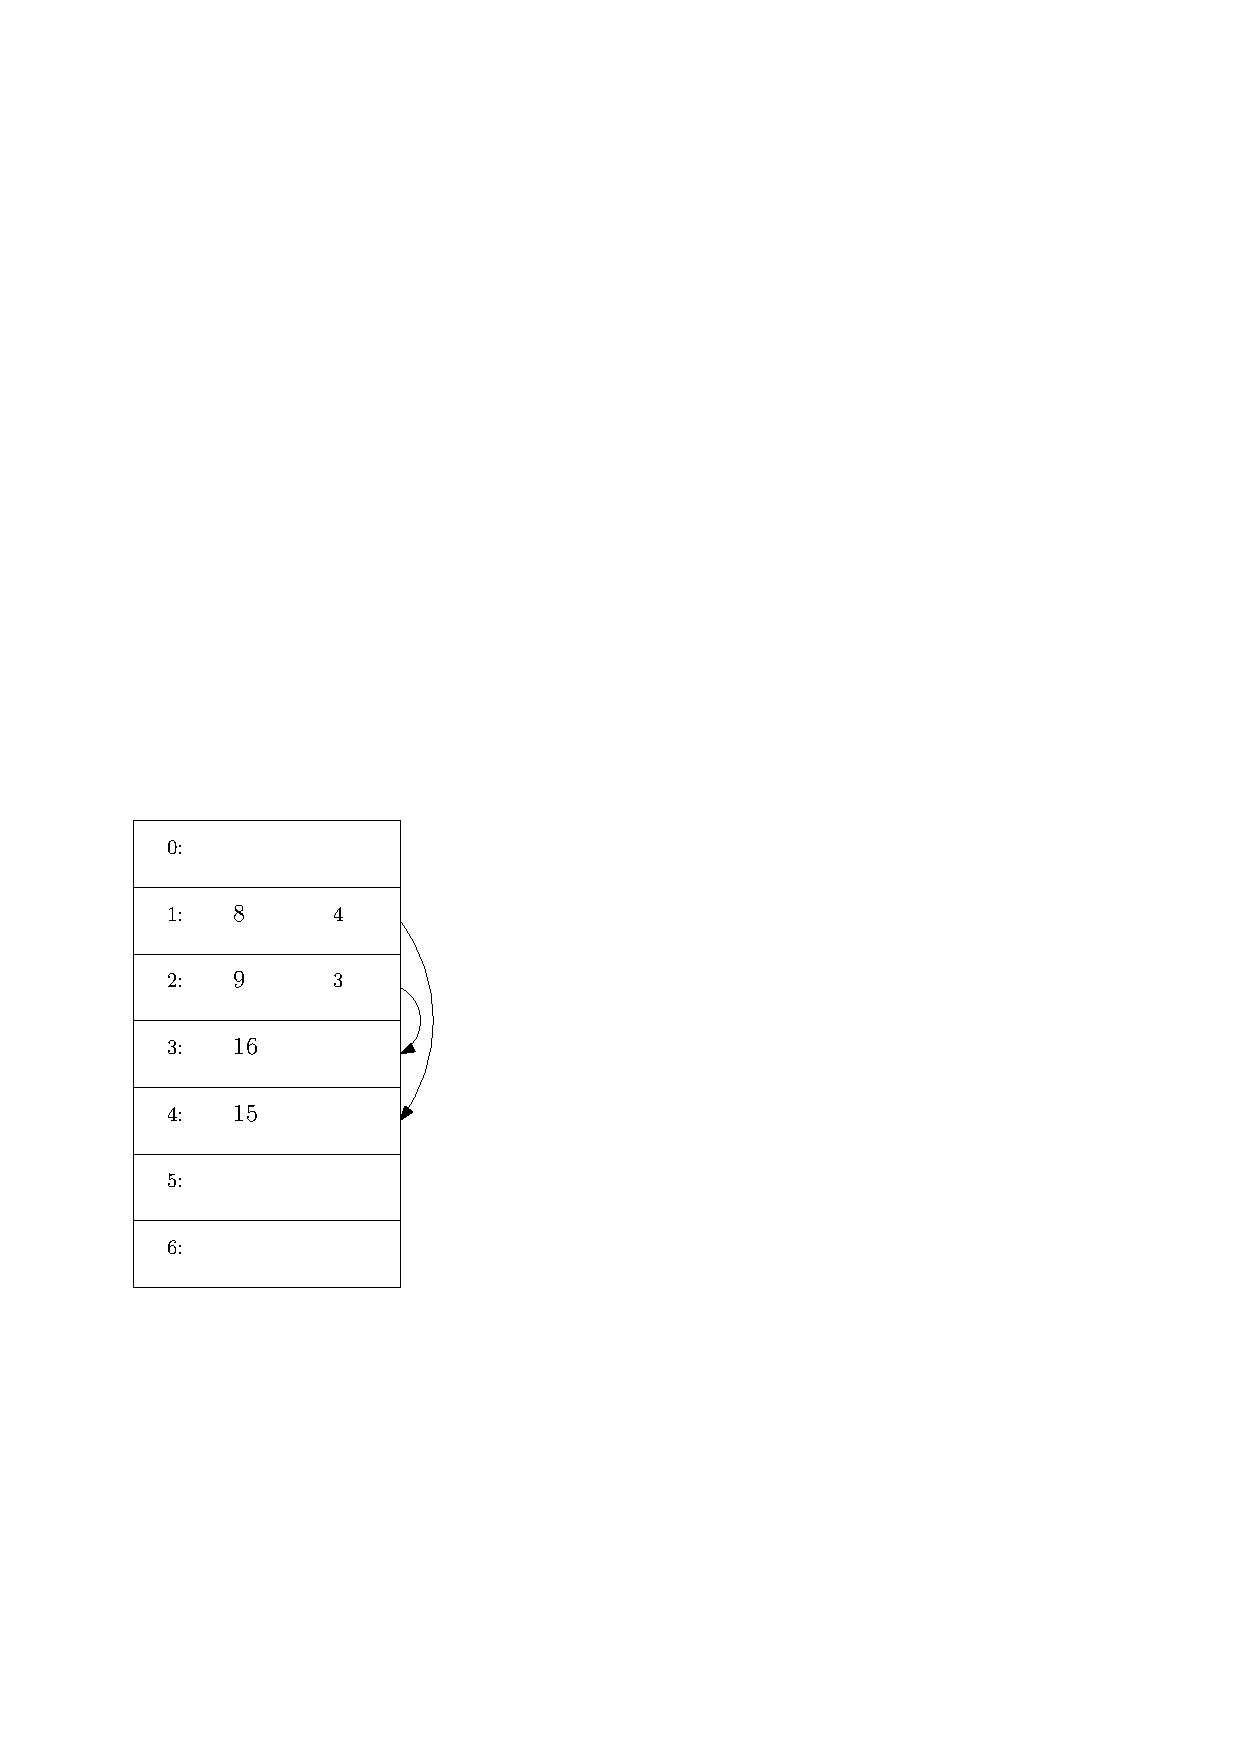
\includegraphics[width=0.2\textwidth]{images/vich}
  \caption{Singly linked lists represented directly in the hash table. The first number is the bucket's address, the second is the represented key and the last one is the next pointer.}
\end{figure}

\section{Open Addressing}
Methods of coalesced hashing and separate chaining represent the chains explicitly by linked lists. The additional pointer of the list not only consumes an extra memory. It also worsens the cache behaviour of the hash table. Open addressing also merges the chains together. They are stored directly in the hash table and their representation is more implicit. To remove the need of an additional pointer, a secondary function for conflict resolution is used.

Models of open addressing assume existence of two hash functions $h_1: U \rightarrow B$ and $h_2: U \rightarrow B$. Assume $x \in U$ is the $i$\textsuperscript{th} element of the chain and the order of elements in a chain starts from zero. Its address is then determined by a compound hash function $h(x, i) = h_1(x) + i h_2(x)$. When we insert the element $x \in U$ we find a minimal $i$ such that the bucket at the address $h(x, i)$ is empty.

This approach also removes the problem of the choice of a free bucket when a collision occurs. Unfortunately, there is no fast implementation of the delete operation known so far. To delete an element we can mark its bucket as free and reuse it when possible. Marking the deleted element's bucket is necessary if we do not want to accidentally loose the elements lying behind the deleted one in the chains.

\subsection{Linear Probing}
Linear probing is a scheme of open addressing with $h_2(x) = 1$ for every $x \in U$. The last element of the prolonged chain is placed into the first empty bucket behind the one with the address $h_1(x)$.

Another problem of linear hashing is its degradation. Clusters of non-empty buckets emerge when load factors reach one. Delete operation implemented by marking only emphasises this problem. Despite of the mentioned problems, linear probing takes the advantage of the good cache behaviour. No wonder, that its modifications are studied nowadays, e.g hopscotch hashing mentioned in Section \ref{section-modern-approaches}.

\subsection{Double Hashing}
If we want to distribute the stored set uniformly across the hash table, then the choice of a free bucket should be random. Whenever function $h(x, i)$ of argument $i$ is a random permutation of $B$, then the mentioned choice becomes random. A necessary condition is that $h_2(x)$ and $m$ are relatively prime. Therefore the size of the hash table is chosen so that it is a prime number again. 

Double hashing has theoretical analyses yielding remarkable results.
\begin{theorem}
Let $\alpha \in (0, 1)$ be the load factor of the hash table resolving collisions by double hashing. Then the running time of the find operation converges to $\frac{1}{1 - \alpha}$ in the unsuccessful case and to $\frac{1}{\alpha}\log\left(\frac{1}{1 - \alpha}\right)$ when the operation is successful.
\end{theorem}
\begin{proof}
The proof is shown in \cite{DBLP:books/sp/Mehlhorn84}.
\end{proof}

\section{Universal Hashing}
Universal hashing uses a universal system of functions instead of a single function. This removes the dependence of universal hashing on the uniformity of its input. It does not require the assumptions of standard hashing made in Section \ref{section-assumptions}. Universal hashing is a randomised algorithm and the probability space is determined by the uniform choice of a hash function, instead of the selection of a stored set. We study universal hashing and its systems in a more detailed way in Chapter \ref{chapter-universal-classes}.

\section{Perfect Hashing}
Assume that the stored set $S$ is known in advance. The problem solved by perfect hashing is how to create a hash table and a hash function such that the find operation takes only a constant time. Insert and delete operations are forbidden, the stored set $S$ remains fixed. Additional requirements are placed on the size of the scheme. Size of the hash table is not the only problem. We must also take care about the space needed to represent the constructed hash function since it becomes quite complex. The problem is solved in \cite{1884}.

\section{Modern Approaches}
\label{section-modern-approaches}
Modern approaches to hashing are nowadays often based on their probabilistic properties. Authors adapt and change their models to improve the asymptotic results in the average case and in the expected worst case. The algorithms still remain fast and are enriched by simple rules. 

Straightforward use of a single function is not enough and various universal systems are used. Theoretical analyses of the models do not necessarily involve the ideas of universal hashing. Universal classes are used as a heuristic. Although the algorithms are not complicated, their analyses become more and more difficult.

A model called \emph{robin hood hashing} \cite{10.1109/SFCS.1985.48}, \cite{Devroye04onworst} is an improvement of the double hashing. In double hashing we are able to access the chain at an arbitrary position in constant time. The main idea of robin hood hashing is to minimise the variance of the expected chain length. If probing starts from the average chain length the expected time of the find operation becomes constant.

Another model, \emph{hopscotch hashing} \cite{DBLP:conf/wdag/HerlihyST08}, is a modification of the linear probing utilising the computer's cache behaviour. A chain is kept together in one place as long as possible. Algorithms in control of the processor cache store whole blocks of memory inside it when only a single part of the block is accessed. Provided that the chains are compact, storing them in the cache is quite probable. This optimisation makes probing substantially faster.

Next investigated model is \emph{cuckoo hashing} \cite{782440}. However, the interest fades these days since there are some problems connected with it \cite{DBLP:conf/sofsem/DietzfelbingerS09}, \cite{1496857}.

\section{Advantages and Disadvantages}
Hashing, compared to other data structures solving the dictionary problem, e.g. trees, does not provide the complete set of operations. If the universe is ordered, we can not query the hash table for the $k$\textsuperscript{th} stored element. The hash functions are supposed to distribute the elements across the table evenly. This assumption is, somehow, in the opposition to the preservation of the ordering. Especially, different functions of a universal class can not preserve the ordering, they are required to be different. So in general, hashing does not provide the operations based or related to ordering, such as $Succ$, $Pred$, $Order$ of an element and the already mentioned operation -- k\textsuperscript{th} stored element. Despite this, it can also be a rare advantage. Trees require an ordering of the elements they store, so when the universe is not naturally ordered a problem occurs. Usually we solve the problem by adding a unique identifier to every element before storing. This consumes a little memory and in distributed environments causes small troubles with uniqueness, too.

The obvious advantage of hashing is its simplicity. In addition, its constant expected time of the find operation may seem far better than the logarithmic time of trees. On the other hand, if provided with an unsuitable, input hashing often degrades. Balanced trees provide warranties for every input they are provided with. This is a tradeoff that has to be decided by the user -- excellent expected and poor worst case time compared to the logarithmic time in every case.

To sum up, when we need a fast and simple to implement mapping of an object to another one, hashing is a good solution. Especially, when the assumptions from Section \ref{section-assumptions} are satisfied. These conditions are often met with objects having artificial identifiers. However, the worst case guarantee is poor. Despite this, the expected worst case warranty is similar to that of trees, as shown later in the work. Nowadays simplicity does not mean any extra advantage. Standard libraries of current programming languages provide us with many implementations of hashing and trees.

